\section{Enigma und Turing Bombe}

\subsection{Historie}
Turing beschäftigte sich bereits vor Beginn des zweiten Weltkriegs mit den Enigma Maschinen, allerdings waren diese von den Italienern und wesentlich simpler wie die Enigma Maschinen später genutzt von den Deutschen. 
Bei Ausbruch des Krieges wurde Turing zusammen mit Neuntausend anderen Spezialisten in den Bletchley Park geholt. Dieser Park wurde zu einer wahren Entschlüsselungsfabrik, in dem später mit Hilfe der 'Bomben' 39 Tausend Enigma Nachrichten im Monat entschlüsselt wurden.

\subsection{Enigma}
Die Enigma Maschine ist eine Verschlüsselungsmaschine, die im zweiten Weltkrieg von den Deutschen genutzt wurde. \\
Bestandteile der Enigma:
\begin{enumerate}
\item Eingabetastatur
\item beleuchtbare Anzeige
\item Steckbrett
\item drei Zahnräder
\end{enumerate}

\subsubsection{Eingabetastatur}
Eine Schreibmaschienenähnliche Tastatur mit allen 26 Buchstaben des Alphabets, in die man die Nachricht eintippen konnte.

\subsubsection{beleuchtbare Anzeige}
Eine Anzeige mit allen 26 Buchstaben des Alphabets, die einzeln beleuchtet werden und die verschlüsselte Nachricht anzeigen z.B ein H wird eingetippt und ein R wird beleuchtet.

\subsubsection{Steckbrett}
Das Steckbrett, welches hinten an der Enigma Maschine angebracht war, diente zur Verschlüsselung, da man hier zehn von 26 Buchstaben manuell miteinander verlinken konnte. Somit wurde z.B. ein eingegebenes A zu einem H und anders herum.

\subsubsection{Zahnräder}
Die Zahnräder dienten zum weiteren Verschlüsseln der Nachrichten und jedes Zahnrad hatte 26 Stufen für jeden Buchstaben des Alphabets. Das Erste Zahnrad, welches die Eingabe passierte drehte sich bei jedem Tastendruck um einen Buchstaben weiter, das zweite Zahnrad mit jedem 26sten Tastendruck und das dritte bei jedem 676sten Tastendruck, also immer wenn das vorige Zahnrad sich einmal komplett gedreht hatte. Diese drei Zahnräder haben dadurch 17.576 (26 x 26 x 26) mögliche Kombinationen.

\subsubsection{Funktion}
Die Enigma Maschine konnte eine Nachricht in 10^16 verschiedenen Weisen verschlüsseln.

\subsubsection{Beispiel}

\begin{figure}[hbtp]
\centering
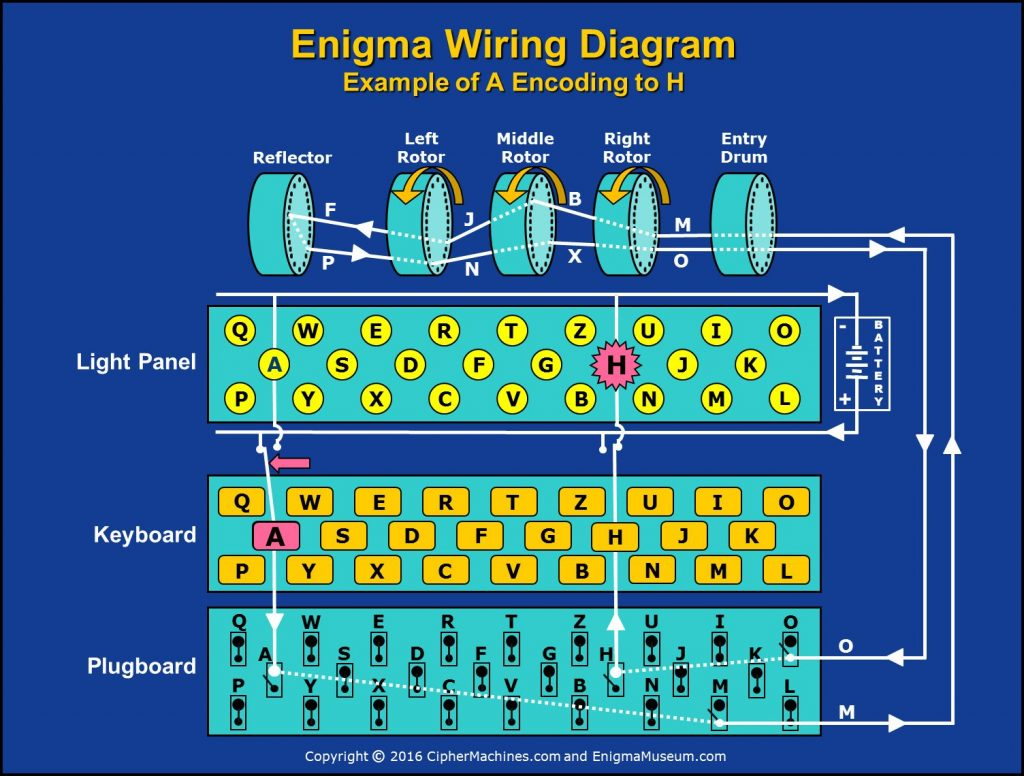
\includegraphics[scale=0.2]{Enigma_Maschine_Beispiel.jpg}
\caption{http://enigmamuseum.com/wp-content/uploads/2016/12/WiringDiagram-1024x776.jpg}
\end{figure}

Der eingegebene Buchstabe A geht erst einmal an das Steckbrett und ist hier mit dem Buchstaben M verbunden. Dieser wird dann an die Zahnräder weitergegeben, die den Buchstaben je nach Stellung verändern, hier von B zu J und schließlich F. Anschließend wird der Buchstabe wieder zurück durch die Zahnräder geleitet und kommt in diesem Beispiel als O heraus und wird wieder an das Steckbrett weitergeleitet. Der Buchstabe O ist hier mit H verbunden und so wird am Ende H in der Anzeige beleuchtet, und somit wurde A zu H verschlüsselt.

\subsection{Turing Bombe}


\subsection{(Bamboo Technik)?}